\documentclass[11pt,]{article}
\usepackage[]{mathpazo}
\usepackage{amssymb,amsmath}
\usepackage{ifxetex,ifluatex}
\usepackage{fixltx2e} % provides \textsubscript
\ifnum 0\ifxetex 1\fi\ifluatex 1\fi=0 % if pdftex
  \usepackage[T1]{fontenc}
  \usepackage[utf8]{inputenc}
\else % if luatex or xelatex
  \ifxetex
    \usepackage{mathspec}
  \else
    \usepackage{fontspec}
  \fi
  \defaultfontfeatures{Ligatures=TeX,Scale=MatchLowercase}
\fi
% use upquote if available, for straight quotes in verbatim environments
\IfFileExists{upquote.sty}{\usepackage{upquote}}{}
% use microtype if available
\IfFileExists{microtype.sty}{%
\usepackage{microtype}
\UseMicrotypeSet[protrusion]{basicmath} % disable protrusion for tt fonts
}{}
\usepackage[margin = 1in]{geometry}
\usepackage{hyperref}
\hypersetup{unicode=true,
            pdfborder={0 0 0},
            breaklinks=true}
\urlstyle{same}  % don't use monospace font for urls
\usepackage{graphicx,grffile}
\makeatletter
\def\maxwidth{\ifdim\Gin@nat@width>\linewidth\linewidth\else\Gin@nat@width\fi}
\def\maxheight{\ifdim\Gin@nat@height>\textheight\textheight\else\Gin@nat@height\fi}
\makeatother
% Scale images if necessary, so that they will not overflow the page
% margins by default, and it is still possible to overwrite the defaults
% using explicit options in \includegraphics[width, height, ...]{}
\setkeys{Gin}{width=\maxwidth,height=\maxheight,keepaspectratio}
\IfFileExists{parskip.sty}{%
\usepackage{parskip}
}{% else
\setlength{\parindent}{0pt}
\setlength{\parskip}{6pt plus 2pt minus 1pt}
}
\setlength{\emergencystretch}{3em}  % prevent overfull lines
\providecommand{\tightlist}{%
  \setlength{\itemsep}{0pt}\setlength{\parskip}{0pt}}
\setcounter{secnumdepth}{0}
% Redefines (sub)paragraphs to behave more like sections
\ifx\paragraph\undefined\else
\let\oldparagraph\paragraph
\renewcommand{\paragraph}[1]{\oldparagraph{#1}\mbox{}}
\fi
\ifx\subparagraph\undefined\else
\let\oldsubparagraph\subparagraph
\renewcommand{\subparagraph}[1]{\oldsubparagraph{#1}\mbox{}}
\fi

%%% Use protect on footnotes to avoid problems with footnotes in titles
\let\rmarkdownfootnote\footnote%
\def\footnote{\protect\rmarkdownfootnote}

%%% Change title format to be more compact
\usepackage{titling}

% Create subtitle command for use in maketitle
\providecommand{\subtitle}[1]{
  \posttitle{
    \begin{center}\large#1\end{center}
    }
}

\setlength{\droptitle}{-2em}

  \title{}
    \pretitle{\vspace{\droptitle}}
  \posttitle{}
    \author{}
    \preauthor{}\postauthor{}
    \date{}
    \predate{}\postdate{}
  
\usepackage{setspace}

\doublespacing
\usepackage[left]{lineno}
\linenumbers
\usepackage{dcolumn}
\usepackage{caption}
\usepackage{float}
\usepackage{afterpage}
\usepackage{siunitx}

\begin{document}

\newpage

\begin{figure}
\centering
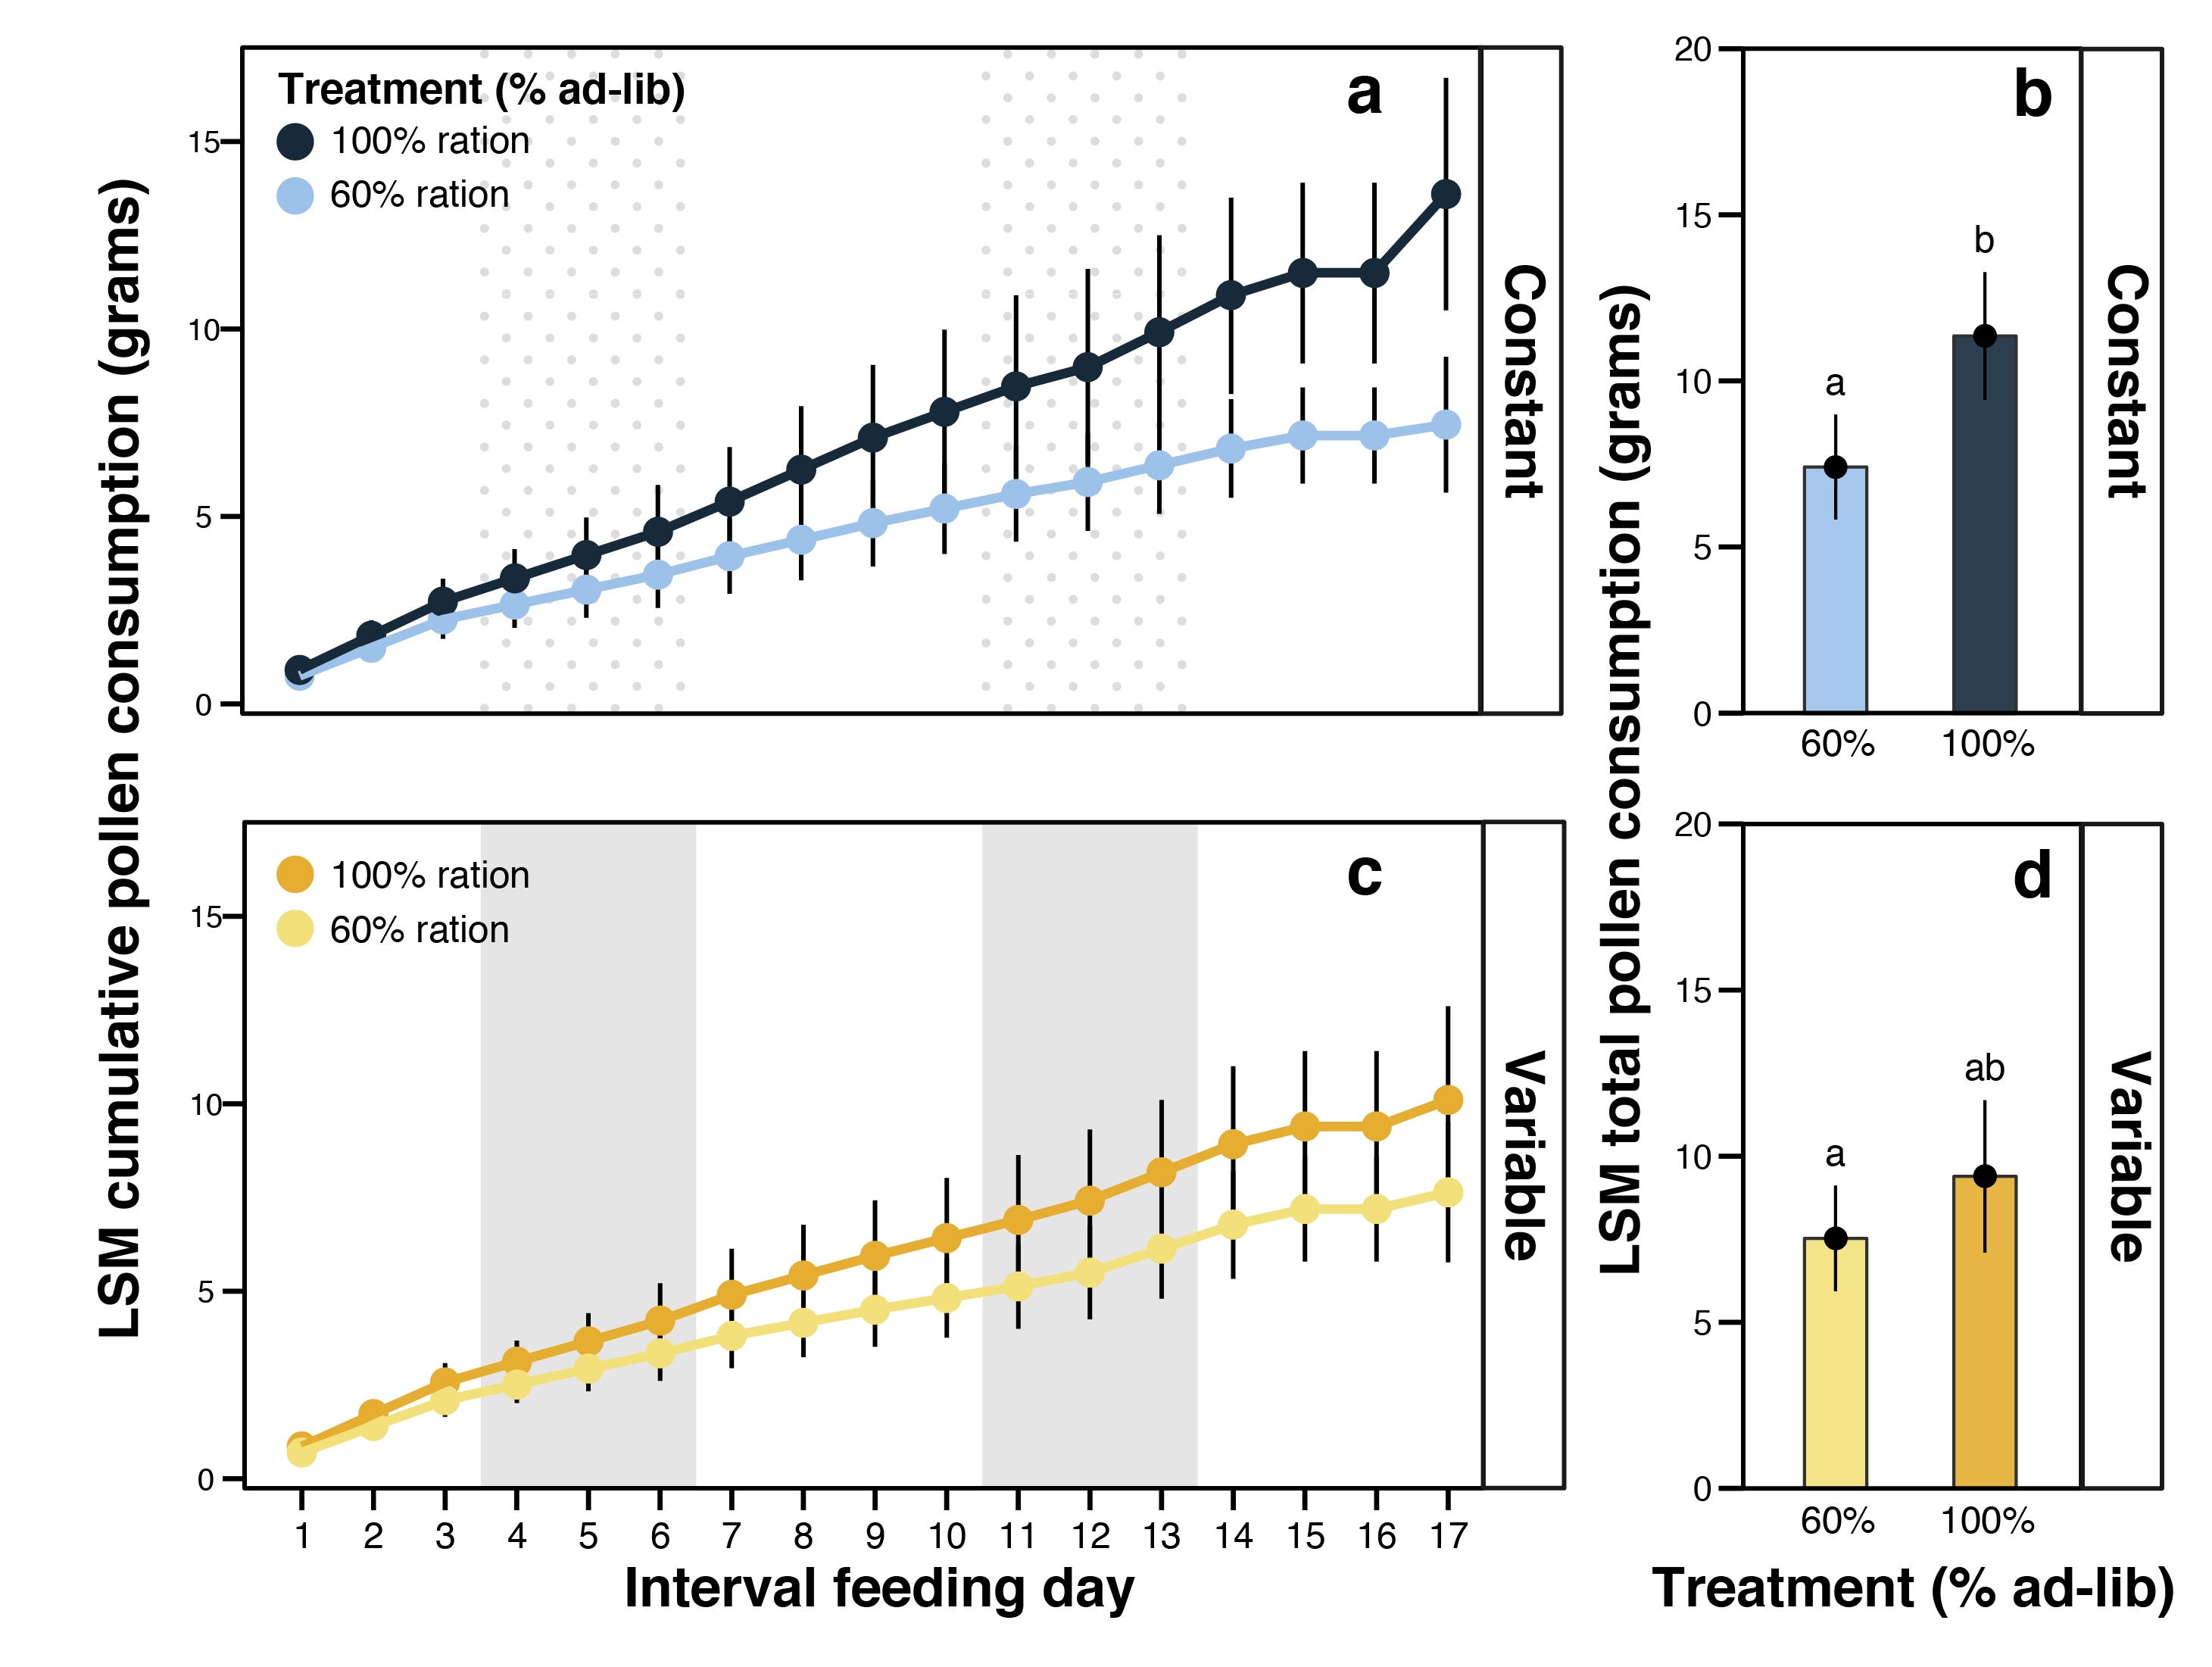
\includegraphics{./supfig1_pollen.png}
\caption{\textbf{Supplemental Figure 1:} (a,c) Least square mean (LSM)
estimated cumulative pollen consumption (b,d) Least square mean total
pollen consumption by treatment. Letters indicate significant
differences both within and across temporal treatment categories
(constant and variable). Error bars are 95\% confidence intervals.
Difference of 1 interval feeding day is equal to 3 Julian days.}
\end{figure}

\clearpage

\begin{figure}
\centering
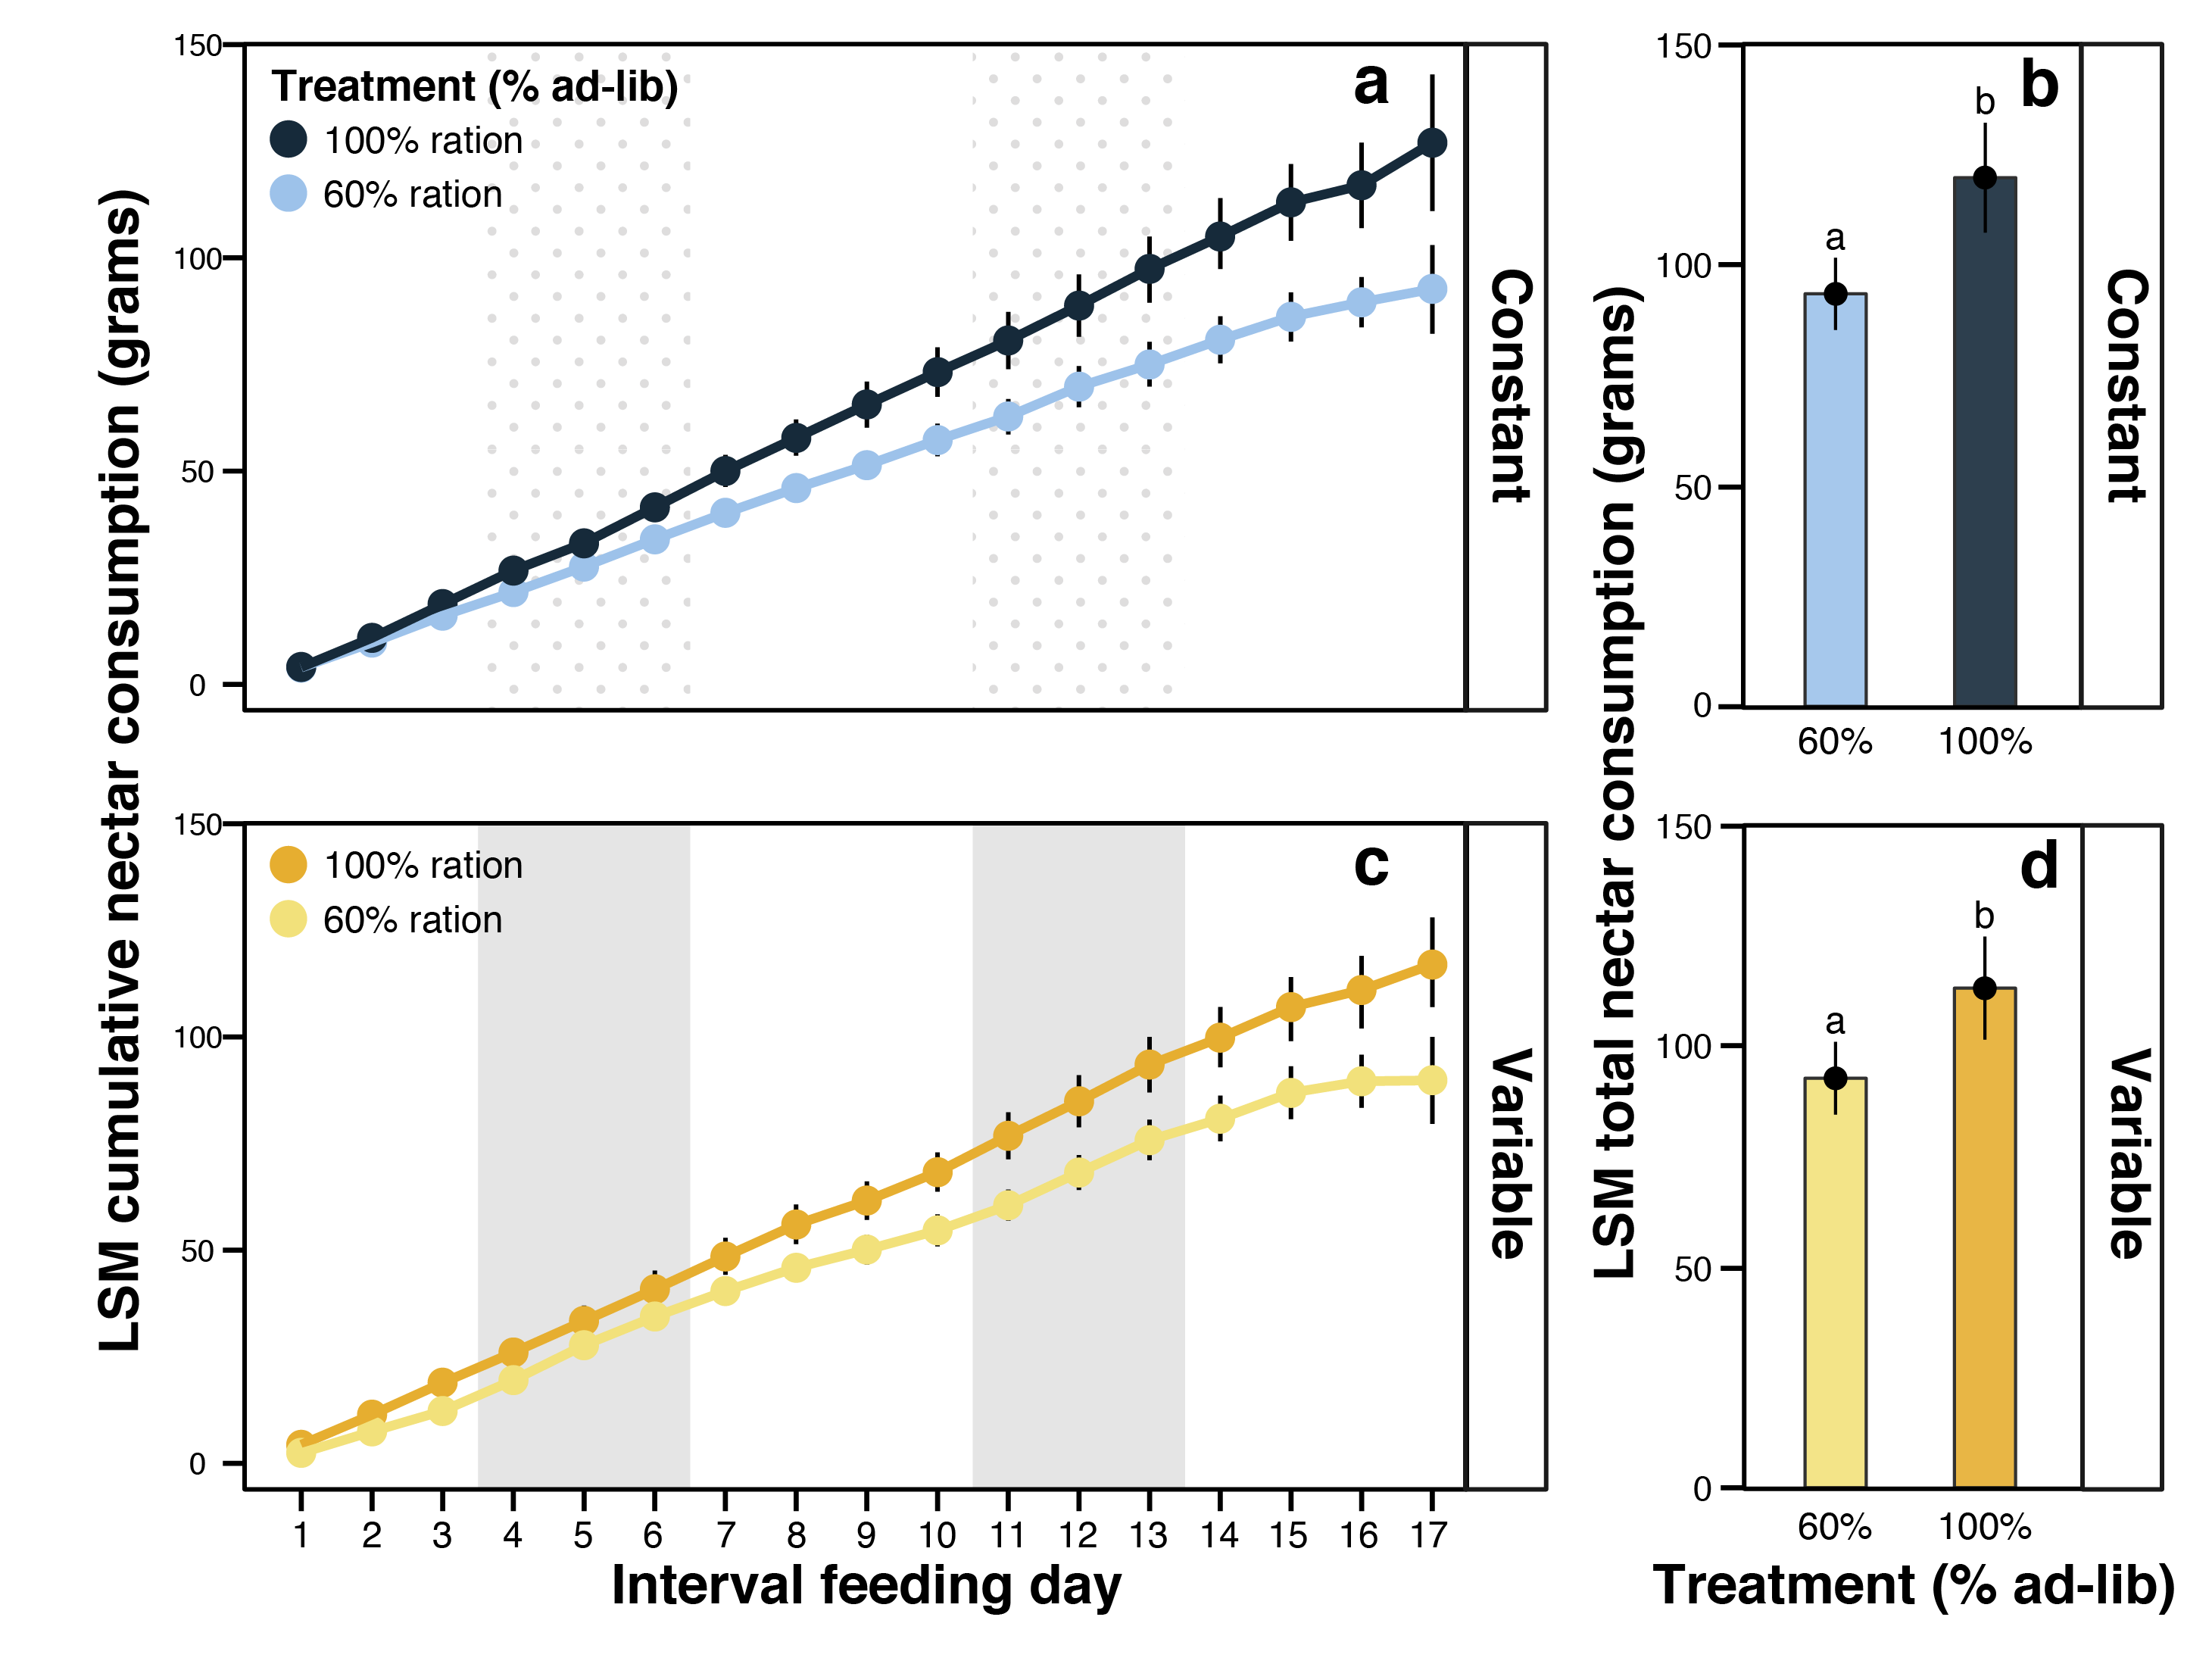
\includegraphics{./supfig2_nectar.png}
\caption{\textbf{Supplemental Figure 2:} (a,c) Least square mean (LSM)
estimated cumulative nectar consumption (b,d) Least square mean total
nectar consumption by treatment. Letters indicate significant
differences both within and across temporal treatment categories
(constant and variable). Error bars are 95\% confidence intervals.
Difference of 1 interval feeding day is equal to 3 Julian days.}
\end{figure}

\clearpage

\newpage
\begin{table}[] \centering
\caption{}{Supplementary Table 1: Mixed model parameter estimates for model with end of experiment microcolony mass as the response variable including 95\% confidence intervals.}
\begin{tabular}{@{\extracolsep{5pt}}lD{.}{.}{-2} }
\\[-1.8ex]\hline
\hline \\[-1.8ex]
 & \multicolumn{1}{c}{\textit{Response Variable:}} \\
\cline{2-2}
\\[-1.8ex] & \multicolumn{1}{c}{Colony Mass} \\
\\[-1.8ex] & \multicolumn{1}{c}{\textit{linear}} \\
 & \multicolumn{1}{c}{\textit{mixed effects}} \\
\hline \\[-1.8ex]
 Intercept & 5.94^{***}$ $(5.04$, $6.85) \\
  Temporal food availability & 1.59^{**}$ $(0.69$, $2.49) \\
  Total food availability & 1.21^{*}$ $(0.30$, $2.11) \\
  Exp. round & -1.26^{***}$ $(-1.67$, $-0.85) \\
  Temporal:Total & 1.18^{*}$ $(0.28$, $2.08) \\
  Temporal:Exp. round & -0.54^{*}$ $(-0.95$, $-0.13) \\
  Total:Exp. round & -0.20$ $(-0.61$, $0.21) \\
  Temporal:Total:Exp. round & -0.38$ $(-0.79$, $0.03) \\
 \hline \\[-1.8ex]
Observations & \multicolumn{1}{c}{80} \\
Log Likelihood & \multicolumn{1}{c}{-147.64} \\
Akaike Inf. Crit. & \multicolumn{1}{c}{315.28} \\
Bayesian Inf. Crit. & \multicolumn{1}{c}{338.05} \\
\hline
\hline \\[-1.8ex]
\textit{Note:}  & \multicolumn{1}{r}{$^{*}$p$<$0.05; $^{**}$p$<$0.01; $^{***}$p$<$0.001} \\
\end{tabular}
\end{table}
\clearpage

\newpage
\begin{table}[] \centering
\caption{}{Supplementary Table 2: Mixed model parameter estimates for model with rate of mass gain as the response variable including 95\% confidence intervals.}
  \label{suptab2}
\begin{tabular}{@{\extracolsep{5pt}}lD{.}{.}{-2} }
\\[-1.8ex]\hline
\hline \\[-1.8ex]
 & \multicolumn{1}{c}{\textit{Response Variable:}} \\
\cline{2-2}
\\[-1.8ex] & \multicolumn{1}{c}{Rate of Mass Gain} \\
\\[-1.8ex] & \multicolumn{1}{c}{\textit{linear}} \\
 & \multicolumn{1}{c}{\textit{mixed effects}} \\
\hline \\[-1.8ex]
 Intercept & 0.21^{***}$ $(0.10$, $0.32) \\
  Temporal food availability & 0.07$ $(-0.04$, $0.18) \\
  Total food availability & 0.13^{*}$ $(0.02$, $0.24) \\
  Time period (before pulse 1) & -0.67^{***}$ $(-0.89$, $-0.45) \\
  Time period (during pulse 1) & -0.40^{***}$ $(-0.62$, $-0.18) \\
  Time period (after pulse 1, before pulse 2) & -0.23^{*}$ $(-0.45$, $-0.01) \\
  Time period (during pulse 2) & -0.14$ $(-0.36$, $0.08) \\
  Temporal:Total & 0.20^{**}$ $(0.09$, $0.31) \\
 \hline \\[-1.8ex]
Observations & \multicolumn{1}{c}{140} \\
Log Likelihood & \multicolumn{1}{c}{-150.53} \\
Akaike Inf. Crit. & \multicolumn{1}{c}{321.06} \\
Bayesian Inf. Crit. & \multicolumn{1}{c}{349.89} \\
\hline
\hline \\[-1.8ex]
\textit{Note:}  & \multicolumn{1}{r}{$^{*}$p$<$0.05; $^{**}$p$<$0.01; $^{***}$p$<$0.001} \\
\end{tabular}
\end{table}
\clearpage

\newpage
\begin{table}[] \centering
\caption{}{Supplementary Table 3: Mixed model parameter estimates for repeated measures model with mass as the response variable including 95\% confidence intervals.}
  \label{}
\begin{tabular}{@{\extracolsep{5pt}}lD{.}{.}{-2} }
\\[-1.8ex]\hline
\hline \\[-1.8ex]
 & \multicolumn{1}{c}{\textit{Response Variable:}} \\
\cline{2-2}
\\[-1.8ex] & \multicolumn{1}{c}{Mass Gain (Temporal trends)} \\
\\[-1.8ex] & \multicolumn{1}{c}{\textit{linear}} \\
 & \multicolumn{1}{c}{\textit{mixed effects}} \\
\hline \\[-1.8ex]
 Intercept & -793.66^{***}$ $(-982.99$, $-604.33) \\
  Total food availability & 1.15^{***}$ $(0.94$, $1.36) \\
  Temporal food availability & 0.13$ $(-0.08$, $0.34) \\
  Exp. round 1 & 4.88^{***}$ $(3.66$, $6.09) \\
  Exp. round 2 & 0.04$ $(-0.33$, $0.41) \\
  date & 0.04^{***}$ $(0.03$, $0.06) \\
  Total:Temporal & 0.19$ $(-0.02$, $0.40) \\
  Total:Exp. round 1 & 0.21$ $(-0.09$, $0.51) \\
  Total:Exp. round 2 & -0.07$ $(-0.37$, $0.23) \\
  Temporal:Exp. round 1 & 0.44^{**}$ $(0.14$, $0.74) \\
  Temporal:Exp. round 2 & -0.27$ $(-0.57$, $0.03) \\
  Total:Temporal:Exp. round 1 & 0.35^{*}$ $(0.06$, $0.65) \\
  Total:Temporal:Exp. round 2 & -0.25$ $(-0.55$, $0.05) \\
 \hline \\[-1.8ex]
Observations & \multicolumn{1}{c}{1,315} \\
Log Likelihood & \multicolumn{1}{c}{-2,589.40} \\
Akaike Inf. Crit. & \multicolumn{1}{c}{5,228.81} \\
Bayesian Inf. Crit. & \multicolumn{1}{c}{5,358.10} \\
\hline
\hline \\[-1.8ex]
\textit{Note:}  & \multicolumn{1}{r}{$^{*}$p$<$0.05; $^{**}$p$<$0.01; $^{***}$p$<$0.001} \\
\end{tabular}
\end{table}
\clearpage

\newpage
\begin{table}[] \centering
\caption{}{Supplementary Table 4: Mixed model parameter estimates for model with cumulative drone production as the response variable including 95\% confidence intervals.}
  \label{}
\begin{tabular}{@{\extracolsep{5pt}}lD{.}{.}{-2} }
\\[-1.8ex]\hline
\hline \\[-1.8ex]
 & \multicolumn{1}{c}{\textit{Response Variable:}} \\
\cline{2-2}
\\[-1.8ex] & \multicolumn{1}{c}{Drone Production} \\
\\[-1.8ex] & \multicolumn{1}{c}{\textit{linear}} \\
 & \multicolumn{1}{c}{\textit{mixed effects}} \\
\hline \\[-1.8ex]
 Intercept & 29.02^{***}$ $(24.92$, $33.12) \\
  Temporal food availability & 2.62$ $(-1.48$, $6.72) \\
  Total food availability & 4.53^{*}$ $(0.43$, $8.63) \\
  rep & -7.43^{***}$ $(-9.29$, $-5.57) \\
  Temporal:Total & 2.70$ $(-1.40$, $6.80) \\
  Temporal:rep & -0.85$ $(-2.70$, $1.01) \\
  Total:rep & -1.05$ $(-2.91$, $0.80) \\
  Temporal:Total:rep & -0.92$ $(-2.78$, $0.94) \\
 \hline \\[-1.8ex]
Observations & \multicolumn{1}{c}{77} \\
Log Likelihood & \multicolumn{1}{c}{-245.15} \\
Akaike Inf. Crit. & \multicolumn{1}{c}{510.30} \\
Bayesian Inf. Crit. & \multicolumn{1}{c}{532.64} \\
\hline
\hline \\[-1.8ex]
\textit{Note:}  & \multicolumn{1}{r}{$^{*}$p$<$0.05; $^{**}$p$<$0.01; $^{***}$p$<$0.001} \\
\end{tabular}
\end{table}
\clearpage

\newpage
\begin{table}[] \centering
\caption{}{Supplementary Table 5: Mixed model parameter estimates for model with time to first drone as the response variable including 95\% confidence intervals.}
  \label{}
\begin{tabular}{@{\extracolsep{5pt}}lD{.}{.}{-2} }
\\[-1.8ex]\hline
\hline \\[-1.8ex]
 & \multicolumn{1}{c}{\textit{Response Variable:}} \\
\cline{2-2}
\\[-1.8ex] & \multicolumn{1}{c}{Time to First Drone} \\
\\[-1.8ex] & \multicolumn{1}{c}{\textit{linear}} \\
 & \multicolumn{1}{c}{\textit{mixed effects}} \\
\hline \\[-1.8ex]
 Intercept & 17.24^{***}$ $(16.12$, $18.35) \\
  Total food availability & -0.50$ $(-1.62$, $0.61) \\
  Temporal food availability & 0.82$ $(-0.29$, $1.94) \\
  Exp. round 1 & -4.18^{***}$ $(-5.47$, $-2.88) \\
  Exp. round 2 & -2.23^{**}$ $(-3.47$, $-0.98) \\
  Total:Temporal & -0.95$ $(-2.07$, $0.17) \\
  Total:Exp. round 1 & -0.63$ $(-1.92$, $0.67) \\
  Total:Exp. round 2 & 0.06$ $(-1.18$, $1.31) \\
  Temporal:Exp. round 1 & 0.19$ $(-1.11$, $1.48) \\
  Temporal:Exp. round 2 & -0.55$ $(-1.80$, $0.70) \\
  Total:Temporal:Exp. round 1 & 1.15$ $(-0.15$, $2.45) \\
  Total:Temporal:Exp. round 2 & 0.24$ $(-1.01$, $1.49) \\
 \hline \\[-1.8ex]
Observations & \multicolumn{1}{c}{75} \\
Log Likelihood & \multicolumn{1}{c}{-204.21} \\
Akaike Inf. Crit. & \multicolumn{1}{c}{436.42} \\
Bayesian Inf. Crit. & \multicolumn{1}{c}{466.42} \\
\hline
\hline \\[-1.8ex]
\textit{Note:}  & \multicolumn{1}{r}{$^{*}$p$<$0.05; $^{**}$p$<$0.01; $^{***}$p$<$0.001} \\
\end{tabular}
\end{table}
\clearpage

\newpage
\begin{table}[] \centering
\caption{}{Supplementary Table 6: Linear model parameter estimates for model with drone mass as the response variable including 95\% confidence intervals.}
  \label{}
\begin{tabular}{@{\extracolsep{5pt}}lD{.}{.}{-2} }
\\[-1.8ex]\hline
\hline \\[-1.8ex]
 & \multicolumn{1}{c}{\textit{Response Variable:}} \\
\cline{2-2}
\\[-1.8ex] & \multicolumn{1}{c}{Drone Mass} \\
\\[-1.8ex] & \multicolumn{1}{c}{\textit{OLS}} \\
\hline \\[-1.8ex]
 Intercept & 0.13^{***}$ $(0.12$, $0.14) \\
  Total food availability & 0.01$ $(-0.001$, $0.02) \\
  Temporal food availability & -0.01$ $(-0.02$, $0.003) \\
  rep & -0.01^{***}$ $(-0.02$, $-0.005) \\
  Total:Temporal & 0.0003$ $(-0.01$, $0.01) \\
  Total:rep & -0.001$ $(-0.01$, $0.005) \\
  Temporal:rep & 0.004$ $(-0.002$, $0.01) \\
  Total:Temporal:rep & -0.0001$ $(-0.01$, $0.01) \\
 \hline \\[-1.8ex]
Observations & \multicolumn{1}{c}{401} \\
R$^{2}$ & \multicolumn{1}{c}{0.06} \\
Adjusted R$^{2}$ & \multicolumn{1}{c}{0.05} \\
Residual Std. Error & \multicolumn{1}{c}{0.05 (df = 393)} \\
F Statistic & \multicolumn{1}{c}{3.87$^{***}$ (df = 7; 393)} \\
\hline
\hline \\[-1.8ex]
\textit{Note:}  & \multicolumn{1}{r}{$^{*}$p$<$0.05; $^{**}$p$<$0.01; $^{***}$p$<$0.001} \\
\end{tabular}
\end{table}
\clearpage

\newpage
\begin{table}[] \centering
\caption{}{Supplementary Table 7: Linear model parameter estimates for model with drone intertegular distance as the response variable including 95\% confidence intervals.}
  \label{}
\begin{tabular}{@{\extracolsep{5pt}}lD{.}{.}{-2} }
\\[-1.8ex]\hline
\hline \\[-1.8ex]
 & \multicolumn{1}{c}{\textit{Response Variable:}} \\
\cline{2-2}
\\[-1.8ex] & \multicolumn{1}{c}{Drone Intertegular Distance} \\
\\[-1.8ex] & \multicolumn{1}{c}{\textit{OLS}} \\
\hline \\[-1.8ex]
 Intercept & 2.89^{***}$ $(2.84$, $2.94) \\
  Total food availability & -0.01$ $(-0.06$, $0.04) \\
  Temporal food availability & 0.001$ $(-0.05$, $0.05) \\
  rep & 0.06^{***}$ $(0.03$, $0.08) \\
  Total:Temporal & -0.03$ $(-0.08$, $0.02) \\
  Total:rep & 0.02$ $(-0.01$, $0.04) \\
  Temporal:rep & 0.01$ $(-0.01$, $0.04) \\
  Total:Temporal:rep & 0.02$ $(-0.01$, $0.04) \\
 \hline \\[-1.8ex]
Observations & \multicolumn{1}{c}{1,163} \\
R$^{2}$ & \multicolumn{1}{c}{0.03} \\
Adjusted R$^{2}$ & \multicolumn{1}{c}{0.02} \\
Residual Std. Error & \multicolumn{1}{c}{0.35 (df = 1155)} \\
F Statistic & \multicolumn{1}{c}{4.85$^{***}$ (df = 7; 1155)} \\
\hline
\hline \\[-1.8ex]
\textit{Note:}  & \multicolumn{1}{r}{$^{*}$p$<$0.05; $^{**}$p$<$0.01; $^{***}$p$<$0.001} \\
\end{tabular}
\end{table}
\clearpage

\newpage
\begin{table}[] \centering
\caption{}{Supplementary Table 8: Mixed model parameter estimates for model with total pollen consumption as the response variable including 95\% confidence intervals.}
  \label{}
\begin{tabular}{@{\extracolsep{5pt}}lD{.}{.}{-2} }
\\[-1.8ex]\hline
\hline \\[-1.8ex]
 & \multicolumn{1}{c}{\textit{Response Variable:}} \\
\cline{2-2}
\\[-1.8ex] & \multicolumn{1}{c}{Total Pollen Consumption} \\
\\[-1.8ex] & \multicolumn{1}{c}{\textit{linear}} \\
 & \multicolumn{1}{c}{\textit{mixed effects}} \\
\hline \\[-1.8ex]
 Intercept & 8.92^{***}$ $(8.25$, $9.60) \\
  Temporal food availability & 0.45$ $(-0.22$, $1.13) \\
  Total food availability & 1.46^{***}$ $(0.78$, $2.13) \\
  Exp. round 1 & 3.77^{***}$ $(2.93$, $4.62) \\
  Exp. round 2 & -1.75^{***}$ $(-2.55$, $-0.95) \\
  Temporal:Total & 0.53$ $(-0.14$, $1.21) \\
  Temporal:Exp. round 1 & 0.43$ $(-0.41$, $1.27) \\
  Temporal:Exp. round 2 & -0.49$ $(-1.29$, $0.31) \\
  Total:Exp. round 1 & 0.98^{*}$ $(0.14$, $1.82) \\
  Total:Exp. round 2 & -0.83^{*}$ $(-1.63$, $-0.03) \\
  Temporal:Total:Exp. round 1 & 0.86$ $(0.02$, $1.71) \\
  Temporal:Total:Exp. round 2 & -0.70$ $(-1.50$, $0.10) \\
 \hline \\[-1.8ex]
Observations & \multicolumn{1}{c}{79} \\
Log Likelihood & \multicolumn{1}{c}{-186.53} \\
Akaike Inf. Crit. & \multicolumn{1}{c}{401.05} \\
Bayesian Inf. Crit. & \multicolumn{1}{c}{431.92} \\
\hline
\hline \\[-1.8ex]
\textit{Note:}  & \multicolumn{1}{r}{$^{*}$p$<$0.05; $^{**}$p$<$0.01; $^{***}$p$<$0.001} \\
\end{tabular}
\end{table}
\clearpage

\newpage
\begin{table}[] \centering
\caption{}{Supplementary Table 9: Mixed model parameter estimates for model with total nectar consumption as the response variable including 95\% confidence intervals.}
  \label{}
\begin{tabular}{@{\extracolsep{5pt}}lD{.}{.}{-2} }
\\[-1.8ex]\hline
\hline \\[-1.8ex]
 & \multicolumn{1}{c}{\textit{Response Variable:}} \\
\cline{2-2}
\\[-1.8ex] & \multicolumn{1}{c}{Total Nectar Consumption} \\
\\[-1.8ex] & \multicolumn{1}{c}{\textit{linear}} \\
 & \multicolumn{1}{c}{\textit{mixed effects}} \\
\hline \\[-1.8ex]
 Intercept & 104.04^{***}$ $(100.47$, $107.61) \\
  Temporal food availability & 1.79$ $(-1.78$, $5.36) \\
  Total food availability & 11.58^{***}$ $(8.01$, $15.15) \\
  Exp. round 1 & 15.96^{***}$ $(11.52$, $20.41) \\
  Exp. round 2 & -6.47^{**}$ $(-10.70$, $-2.25) \\
  Temporal:Total & 1.56$ $(-2.01$, $5.13) \\
  Temporal:Exp. round 1 & 2.42$ $(-2.03$, $6.86) \\
  Temporal:Exp. round 2 & -1.51$ $(-5.73$, $2.72) \\
  Total:Exp. round 1 & 2.60$ $(-1.85$, $7.05) \\
  Total:Exp. round 2 & -4.45^{*}$ $(-8.67$, $-0.22) \\
  Temporal:Total:Exp. round 1 & 2.96$ $(-1.49$, $7.40) \\
  Temporal:Total:Exp. round 2 & 0.26$ $(-3.97$, $4.48) \\
 \hline \\[-1.8ex]
Observations & \multicolumn{1}{c}{79} \\
Log Likelihood & \multicolumn{1}{c}{-298.10} \\
Akaike Inf. Crit. & \multicolumn{1}{c}{624.20} \\
Bayesian Inf. Crit. & \multicolumn{1}{c}{655.07} \\
\hline
\hline \\[-1.8ex]
\textit{Note:}  & \multicolumn{1}{r}{$^{*}$p$<$0.05; $^{**}$p$<$0.01; $^{***}$p$<$0.001} \\
\end{tabular}
\end{table}
\clearpage

\newpage
\begin{table}[] \centering
\caption{}{Supplementary Table 10: Mixed model parameter estimates for model with total worker mortality as the response variable including 95\% confidence intervals.}
  \label{}
\begin{tabular}{@{\extracolsep{5pt}}lD{.}{.}{-2} }
\\[-1.8ex]\hline
\hline \\[-1.8ex]
 & \multicolumn{1}{c}{\textit{Response Variable:}} \\
\cline{2-2}
\\[-1.8ex] & \multicolumn{1}{c}{Total Worker Mortality} \\
\\[-1.8ex] & \multicolumn{1}{c}{\textit{linear}} \\
 & \multicolumn{1}{c}{\textit{mixed effects}} \\
\hline \\[-1.8ex]
 Intercept & 8.94^{***}$ $(7.73$, $10.14) \\
  Temporal food availability & -0.12$ $(-1.33$, $1.09) \\
  Total food availability & -0.12$ $(-1.33$, $1.08) \\
  Exp. round 1 & -1.17$ $(-2.92$, $0.59) \\
  Exp. round 2 & -3.15^{***}$ $(-4.82$, $-1.48) \\
  Temporal:Total & 0.41$ $(-0.80$, $1.61) \\
  Temporal:Exp. round 1 & -1.28$ $(-3.03$, $0.47) \\
  Temporal:Exp. round 2 & 0.83$ $(-0.84$, $2.51) \\
  Total:Exp. round 1 & -0.004$ $(-1.76$, $1.75) \\
  Total:Exp. round 2 & 0.41$ $(-1.26$, $2.08) \\
  Temporal:Total:Exp. round 1 & 1.49$ $(-0.26$, $3.24) \\
  Temporal:Total:Exp. round 2 & -1.19$ $(-2.87$, $0.48) \\
 \hline \\[-1.8ex]
Observations & \multicolumn{1}{c}{79} \\
Log Likelihood & \multicolumn{1}{c}{-232.32} \\
Akaike Inf. Crit. & \multicolumn{1}{c}{492.64} \\
Bayesian Inf. Crit. & \multicolumn{1}{c}{523.50} \\
\hline
\hline \\[-1.8ex]
\textit{Note:}  & \multicolumn{1}{r}{$^{*}$p$<$0.05; $^{**}$p$<$0.01; $^{***}$p$<$0.001} \\
\end{tabular}
\end{table}
\clearpage

\newpage
\begin{table}[] \centering
\caption{}{Supplementary Table 11: Mixed model parameter estimates for model with pollen per drone produced as the response variable including 95\% confidence intervals.}
  \label{}
\begin{tabular}{@{\extracolsep{5pt}}lD{.}{.}{-2} }
\\[-1.8ex]\hline
\hline \\[-1.8ex]
 & \multicolumn{1}{c}{\textit{Response Variable:}} \\
\cline{2-2}
\\[-1.8ex] & \multicolumn{1}{c}{Pollen per Drone} \\
\\[-1.8ex] & \multicolumn{1}{c}{\textit{linear}} \\
 & \multicolumn{1}{c}{\textit{mixed effects}} \\
\hline \\[-1.8ex]
 Intercept & 0.70^{***}$ $(0.64$, $0.77) \\
  Temporal food availability & 0.01$ $(-0.06$, $0.08) \\
  Total food availability & -0.01$ $(-0.08$, $0.06) \\
  Exp. round 1 & -0.16^{**}$ $(-0.26$, $-0.06) \\
  Exp. round 2 & -0.002$ $(-0.10$, $0.09) \\
  Temporal:Total & -0.07$ $(-0.14$, $0.002) \\
  Temporal:Exp. round 1 & -0.03$ $(-0.13$, $0.07) \\
  Temporal:Exp. round 2 & 0.05$ $(-0.05$, $0.14) \\
  Total:Exp. round 1 & 0.01$ $(-0.08$, $0.11) \\
  Total:Exp. round 2 & -0.06$ $(-0.15$, $0.04) \\
  Temporal:Total:Exp. round 1 & 0.09$ $(-0.004$, $0.19) \\
  Temporal:Total:Exp. round 2 & -0.04$ $(-0.13$, $0.06) \\
 \hline \\[-1.8ex]
Observations & \multicolumn{1}{c}{73} \\
Log Likelihood & \multicolumn{1}{c}{-36.08} \\
Akaike Inf. Crit. & \multicolumn{1}{c}{100.15} \\
Bayesian Inf. Crit. & \multicolumn{1}{c}{129.70} \\
\hline
\hline \\[-1.8ex]
\textit{Note:}  & \multicolumn{1}{r}{$^{*}$p$<$0.05; $^{**}$p$<$0.01; $^{***}$p$<$0.001} \\
\end{tabular}
\end{table}
\clearpage

\newpage
\begin{table}[] \centering
\caption{}{Supplementary Table 12: Mixed model parameter estimates for model with nectar per drone produced as the response variable including 95\% confidence intervals.}
  \label{}
\begin{tabular}{@{\extracolsep{5pt}}lD{.}{.}{-2} }
\\[-1.8ex]\hline
\hline \\[-1.8ex]
 & \multicolumn{1}{c}{\textit{Response Variable:}} \\
\cline{2-2}
\\[-1.8ex] & \multicolumn{1}{c}{Nectar per Drone} \\
\\[-1.8ex] & \multicolumn{1}{c}{\textit{linear}} \\
 & \multicolumn{1}{c}{\textit{mixed effects}} \\
\hline \\[-1.8ex]
 Intercept & 9.89^{***}$ $(8.55$, $11.22) \\
  Temporal food availability & -0.31$ $(-1.65$, $1.03) \\
  Total food availability & 0.09$ $(-1.24$, $1.43) \\
  Exp. round 1 & -4.20^{***}$ $(-6.12$, $-2.28) \\
  Exp. round 2 & 1.52$ $(-0.33$, $3.38) \\
  Temporal:Total & -1.75^{*}$ $(-3.09$, $-0.41) \\
  Temporal:Exp. round 1 & 0.06$ $(-1.86$, $1.98) \\
  Temporal:Exp. round 2 & 0.63$ $(-1.23$, $2.48) \\
  Total:Exp. round 1 & -0.44$ $(-2.36$, $1.47) \\
  Total:Exp. round 2 & -0.32$ $(-2.17$, $1.54) \\
  Temporal:Total:Exp. round 1 & 1.55$ $(-0.37$, $3.47) \\
  Temporal:Total:Exp. round 2 & -0.20$ $(-2.06$, $1.65) \\
 \hline \\[-1.8ex]
Observations & \multicolumn{1}{c}{73} \\
Log Likelihood & \multicolumn{1}{c}{-217.06} \\
Akaike Inf. Crit. & \multicolumn{1}{c}{462.12} \\
Bayesian Inf. Crit. & \multicolumn{1}{c}{491.67} \\
\hline
\hline \\[-1.8ex]
\textit{Note:}  & \multicolumn{1}{r}{$^{*}$p$<$0.05; $^{**}$p$<$0.01; $^{***}$p$<$0.001} \\
\end{tabular}
\end{table}
\clearpage


\end{document}
